\documentclass[12pt]{article}
\usepackage[margin=1.15in]{geometry}
\usepackage[english]{babel}
\usepackage[utf8x]{inputenc}
\usepackage{amsmath}
\usepackage{amsfonts}
\newcommand{\ts}{\textsuperscript}
\usepackage{enumerate}
\usepackage{hyperref}
\usepackage[normalem]{ulem}
\usepackage{graphicx}
\setlength{\parindent}{0in}
\usepackage{color}

\begin{document}
\begin{center}
\begin{Large} Chord Root Prediction Using Supervised Classification Models \end{Large}
\end{center}


\section{Introduction}
Chord roots are an essential construct in tonal music. They can be ambiguous, however, and whether a certain chord exists at a particular time is often up to human interpretation. Nevertheless, there are a multitude of factors which can help in building automated prediction models which emulate human-annotated progression markings with high precision. I built various models and tested their effectiveness in predicting the chords in various Bach Chorales.


\section{Methodology}
\subsection{Data}
I used a set of Bach Chorales as my data set, retrieved and translated by Craig through KernScores [REF]. 70 chorales were analyzed altogether, giving 5206 data points of pitch collections for use in analysis. They are short in length, but contain rich, complex chord sequences ripe for analysis. Chords have been given human annotations, and the key of the song has been determined, or a reasonable estimation has been made. \\

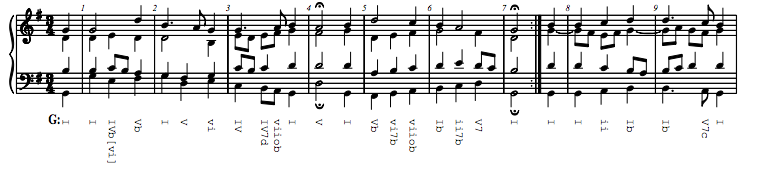
\includegraphics[trim = 0.5cm 0 0 0, scale=0.65]{staff.png}
\begin{center}\emph{Figure 1: Excerpt from Aus meines Herzens Grunde}\\ \end{center}

\begin{color}{white}.\end{color}\\Sheet music was translated into CSV files, listing the sequences of unique pitch collections, and their locations and durations in the music. \\

\begin{center}
  \begin{tabular}{ c | c | c | c || c | c }
    Bar & Beat & Key & Pitches & Chord & Harmony\\
    0 & 3 & G & 1d, 2g, 1b & G & I\\ \hline
    1 & 1 & G & 1d, 2g, 1b & G & I\\ \hline
    1 & 2 & G & 1c, 2e, 1g & E & IVb[vi]\\ \hline
    1  & 2.5 & G & 2e, 1g, 1b & E & (IVb[vi])\\ \hline
    1 & 3 & G & 2d, 1f\#, 1a & D & Vb \\
  \end{tabular}
\end{center}
\begin{center}\emph{Data representation of first two bars from (fig 1)}\\ \end{center}
\newpage

\subsection{Classifiers}
I used probabilistic classification models, or classifiers, to predict chords corresponding to each pitch collection. Classifiers work by analyzing a set of data points $$\mathcal{D} = \{(X_0,y_0), (X_1,y_1), ... (X_n,y_n)\},$$ where $X_i$ is a pitch collection (point), and $y_i$ is the corresponding chord (label). Features $F(X_i) = \{f_0(X_i), f_1(X_i), ..., f_k(X_i)\}$ are extracted from each point - the definition of a feature is rather arbitrary, and it is ultimately up to the developer to come up with meaningful features for the data. The classifier then trains itself on $\mathcal{D}$, assigning weights to the features depending on their usefulness in determining $y_i$. Once trained, the classifier, on a new data point $(X_j,y_j)$, extracts the features from $X_j$, applies the weights as determined by training, and predicts the value of $y_j$ based on the calculated value. 

\subsubsection{Naive Bayes}
Naive Bayes is a simple probabilistic classifier, called ``naive" because it treats each feature independently - it has nevertheless been shown to be effective in practice. Say the set of possible chords is $C$, and the set of input features are $F$. The classifier then works on the following model: 
$$c = \arg \max_{c \in C} P(c) \prod_{f \in F} P(f|c)$$

It can be seen then, that Naive Bayes works by flagging the \emph{existence} of a feature, rather than by measuring a gradient or integer value. This has the potential to be effective here, since a set of pitches can be independently inputted into the system. Naive Bayes is not, however, able to recognize \emph{combinations} of features, such as the significance of having the pitches \texttt{(d,f\#,a)} inputted together (though this can be separately added as an independent feature).

\subsubsection{SVM}
Support Vector Machines (SVM) are a type of \emph{linear binary classifier}, making classifications by mapping features to a geometrical space and determining a hyperplane which splits labelled points into two regions. An input data point is then classified based on the region it falls into. Say the hyperplane is $(\bold{w},b)$, where $\bold{w}$ is the set of feature weights and $b$ is a bias value. Then, given an input point $X$, 
$$y_{pred} = \text{sign}(\bold{w} \cdot F(X) - b),$$

where $F(X)$ is the set of features extracted from $X$. SVM has the advantage of allowing features to complement one another during training due to the geometrical interpretation. Features can simply be mapped to numerical values (\texttt{a\# = 1}, for example) to allow for this. SVM comes with the disadvantage of being a binary classifier, however, meaning multi-classification problems need to be solved through a sequence of binary classifications; this is generally not a significant problem, however.

\subsubsection{k Nearest Neighbors}
$k$ Nearest Neighbors (kNN) is a simple geometrical classifier, classifying a given point $p$ based on the labels assigned to the $k$ nearest points, weighed based on their distance from $p$. It uses the same feature representation as SVM. Though generally less effective than SVM, it has the advantage of being non-linear, and allowing classifications in a space for which no theoretical hyperplane exists.

\subsection{Features}
Feature selection is at the heart of the classification problem - meaningful features are necessary for high precision classifiers. I extracted five main types of features in my analysis.

\subsubsection{Pitches}

These are simply the pitches obtained from the data. In Naive Bayes, if a pitch exists in the data, a feature is constructed notifying its existence. The pitch data comes with occurence counts; if the count is greater than 1, an additional feature is constructed notifying this as well. In the SVM model, each pitch is simply attributed its occurence count (0 if a pitch is not listed in the data). \\


\texttt{NB:  1d, 2g, 1b => [d, g, b, Strong-g]}\\
\texttt{SVM:  1d, 2g, 1b => [a-:0, a:0, a\#:0, ..., b:1, ..., d:1, ..., g:2, g\#:0]}

\subsubsection{Stacks of Thirds}
Stacks of Thirds is a root-estimation method which calculates how closely a set of pitches corresponds to a pitch class $\{A,B,C,D,E,F,G\}$ [REF]. For each class, pitches are scored based on their distance from the base pitch in measurements of thirds. For each third-distance from the base pitch, the score (starting from 0) assigned for the class increases by one - a low score is ultimately desirable. 

\begin{center}
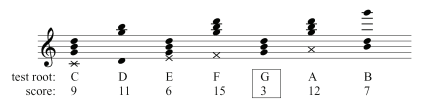
\includegraphics[trim = 0 0 0 0, scale=0.65]{stackOfThirds.png}
\end{center}
\begin{center}\emph{Figure 2: Stack of Thirds scores for (d,g,b). Borrowed from [REF]}\\ \end{center}

In Naive Bayes, the classes with the three lowest overall scores are returned. In SVM, all scores are returned.\\

\texttt{NB:  1d, 2g, 1b => [best-root:G, snd-best-root:E, thd-best-root:B]}\\
\texttt{SVM:  1d, 2g, 1b => [C:9, D:11, E:6, F:15, G:3, A:12, B:7]}


\subsubsection{Major/Minor Triads}
Major/Minor triads are a more direct representation of the Stacks of Thirds feature. It takes, for any chord root, the set of major and minor triads - $\{C,E,E-,G\}$ for Cmaj, for example - and returns a score representing the intersection of the pitches in the chord root, and the pitches in the time slice. 

\texttt{NB: 1d, 2g, 1b => [best-mm: G, snd-best-mm: B, thd-best-mm: D]}\\
\texttt{SVM: 1d, 2g, 1b => [C: 0, D: 1, E: 1, F: 0, G: 3,  A: 0, B: 2]}
\subsubsection{Sliding Window}
The time dependance of the data allows us to see the preceding and subsequent time slices for any given slice - sliding windows consists of including as features, for any time slice, the pitches from the previous and subsequent slices as well. This window can be expanded as needed - a window size of 0 indicates no window at all.
\begin{center}
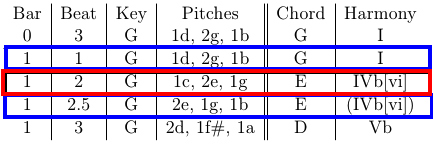
\includegraphics[trim = 0.5cm 0 0 0, scale=0.65]{slice.png}
\end{center}
\begin{center}\emph{Figure 3: The third time slice includes in its features the pitch data from the second and fourth slices.}\\ \end{center}

\subsubsection{Markov Chains}
Markov chains are mathematical systems which undergo transitions from one state to another on a state space, given a random probability distribution for each transition. Craig returned common progressions for me from the Bach Chorales, and I used these to calculate 1st, 2nd, and 3rd order Markov transition matrices. The markov prediction for a given time slice was then calculated as such:\\

For the $k$th order Markov chain, the root scores of the $k$ previous time slices are calculated. The set of possible $k$-length recorded progressions is retrieved, and a score is applied to each progression, which is the sum of the root scores applied for each, based on the key of the time slice. For the progression I IV I, and the key is C, then the score for the progression is the sum of the root scores for C in the first progression, F in the second, and C in the third. The progression with the lowest score is selected. This progression has a distribution of destination chord roots - a score is attached to each destination, representing the product of the probability of the destination, and the associated root score for the current time slice. If the destination is V, and the key is C, then the score for V is the probability of the transition to V multiplied by the root score in the current time slice for G.

\section{Results}
\begin{center}
  \begin{tabular}{ c | c  c | c  c | c c}
    & NB Acc & NB Var & SVM Acc & SVM Var & kNN Acc & kNN Var \\ \hline
   Pitches & 0.799 & 2.09e-5 & 0.884 & 2.30e-5 & 0.893 & 1.10e-4\\	
Stacks of Thirds & 0.868 & 1.17e-4 & 0.889 & 3.20e-5 & 0.895 & 4.94e-5\\	
Major/Minor Triads & 0.795 & 1.48e-4 & 0.811 & 1.98e-5 & 0.783 & 4.86e-4\\	
Sliding Window & 0.809 & 8.54e-5 & 0.892 & 3.80e-5 & 0.892 & 1.86e-5\\	
Markov Chains & 0.343 & 2.05e-4 & 0.423 & 2.42e-4 & 0.359 & 1.69e-4\\ \hline
Combined & 0.900 & 4.46e-5 & 0.909 & 5.78e-5 & 0.883 & 1.25e-4\\	
  \end{tabular}
\end{center}
\begin{center}\emph{Figure 4: Accuracies and variance calculations for each classifier and individual feature, along with the scores obtained when all features are combined. 10 trials were averaged for each.}\\ \end{center}
All three classifiers averaged close to 90\%, with the kNN classifier underperforming and the SVM classifier overperforming. It can be noticed that the Stacks of Thirds feature was especially close to achieving the combined estimation in each classifier, with the other features only increasing accuracy by a few percentage points afterwards. The Markov Chains were notably ineffective in producing results, with accuracies well below 50\%. Sliding window trial runs recorded higher accuracies then the simple pitch estimations, as expected. Major/minor triads achieved poorer results overall than the Stacks of Thirds.\\

The results hint that the features outside of Stacks of Thirds are failing to capture extra insight into what the chord root for the time slice may be. I assumed, initially, that the Sliding Window and Markov Chains features would be able to capture information outside the immediate time slice, but they did not increase total scores as much as I would have expected. \\

Some further insight into the incorrect classifications shows that there is a consistency in the wrongly categorized roots, indicating that a proper feature may boost the accuracy by several percentage points.


\newpage
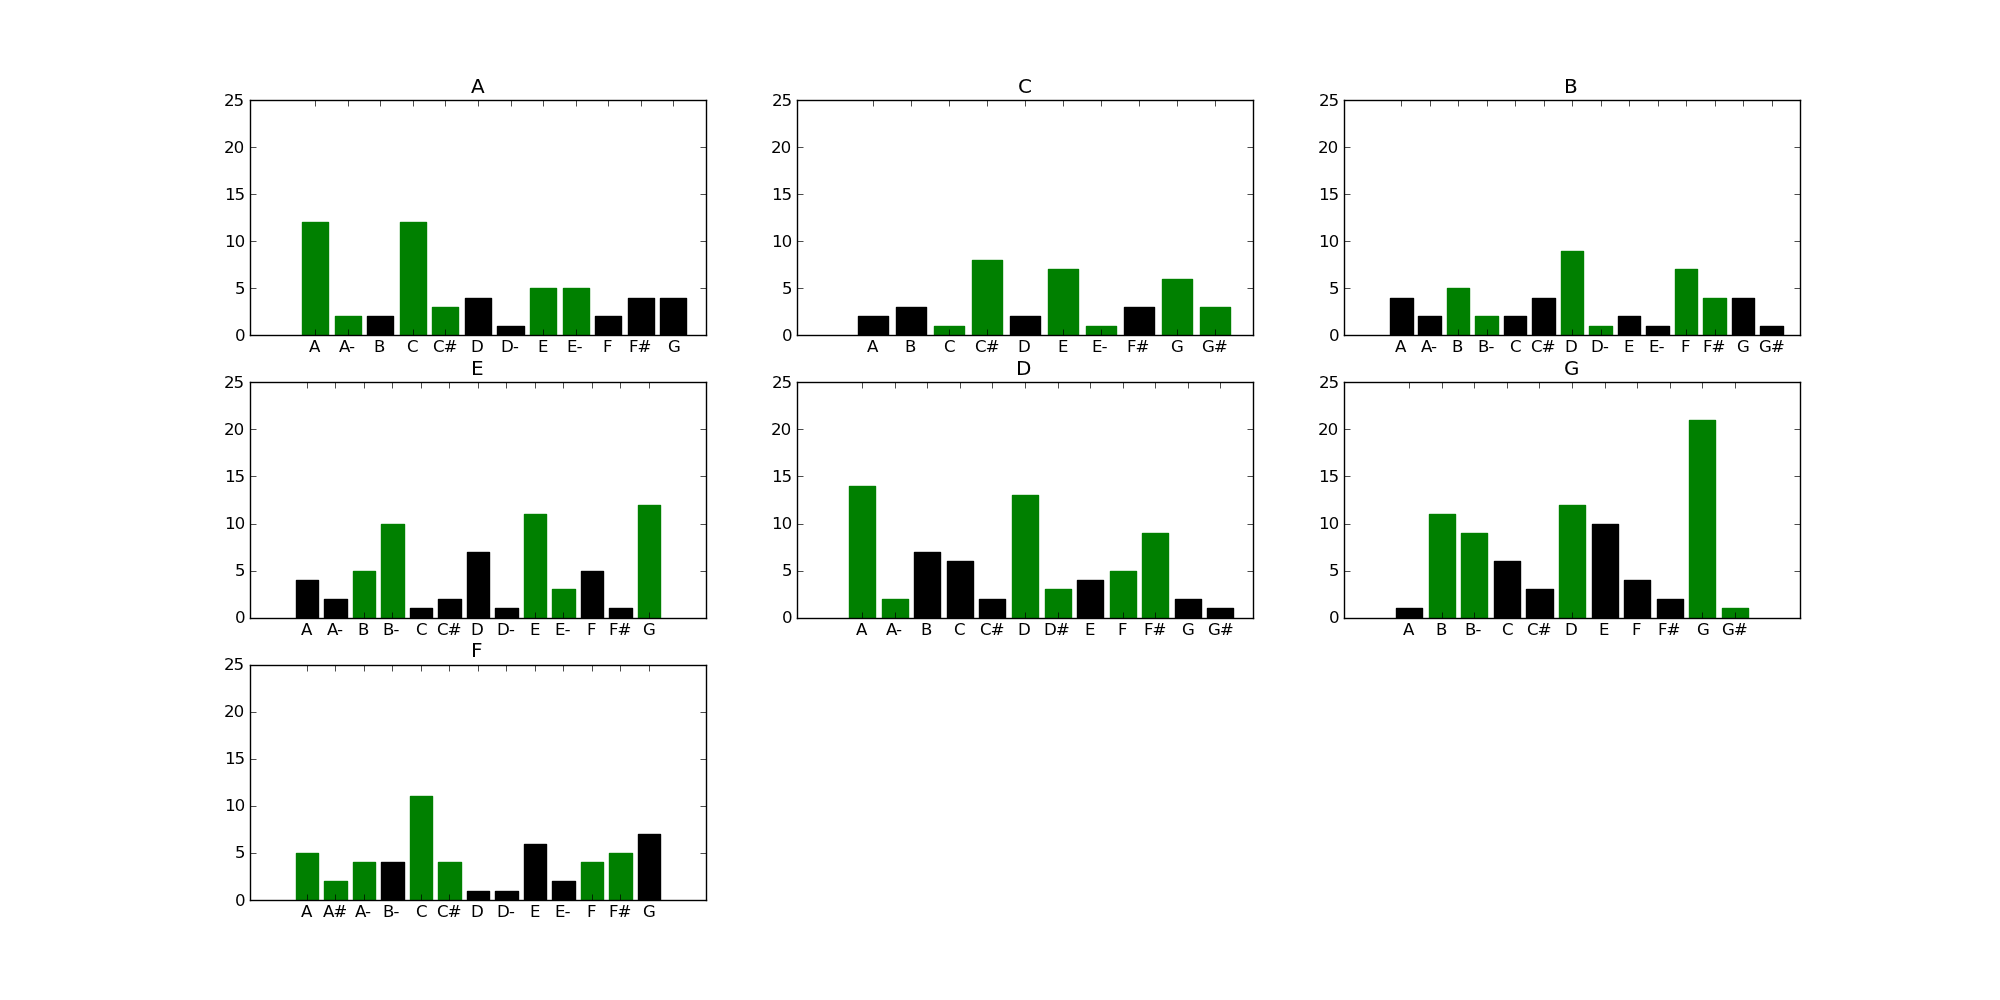
\includegraphics[trim = 220 50 0 30, scale=.45]{actual.png}
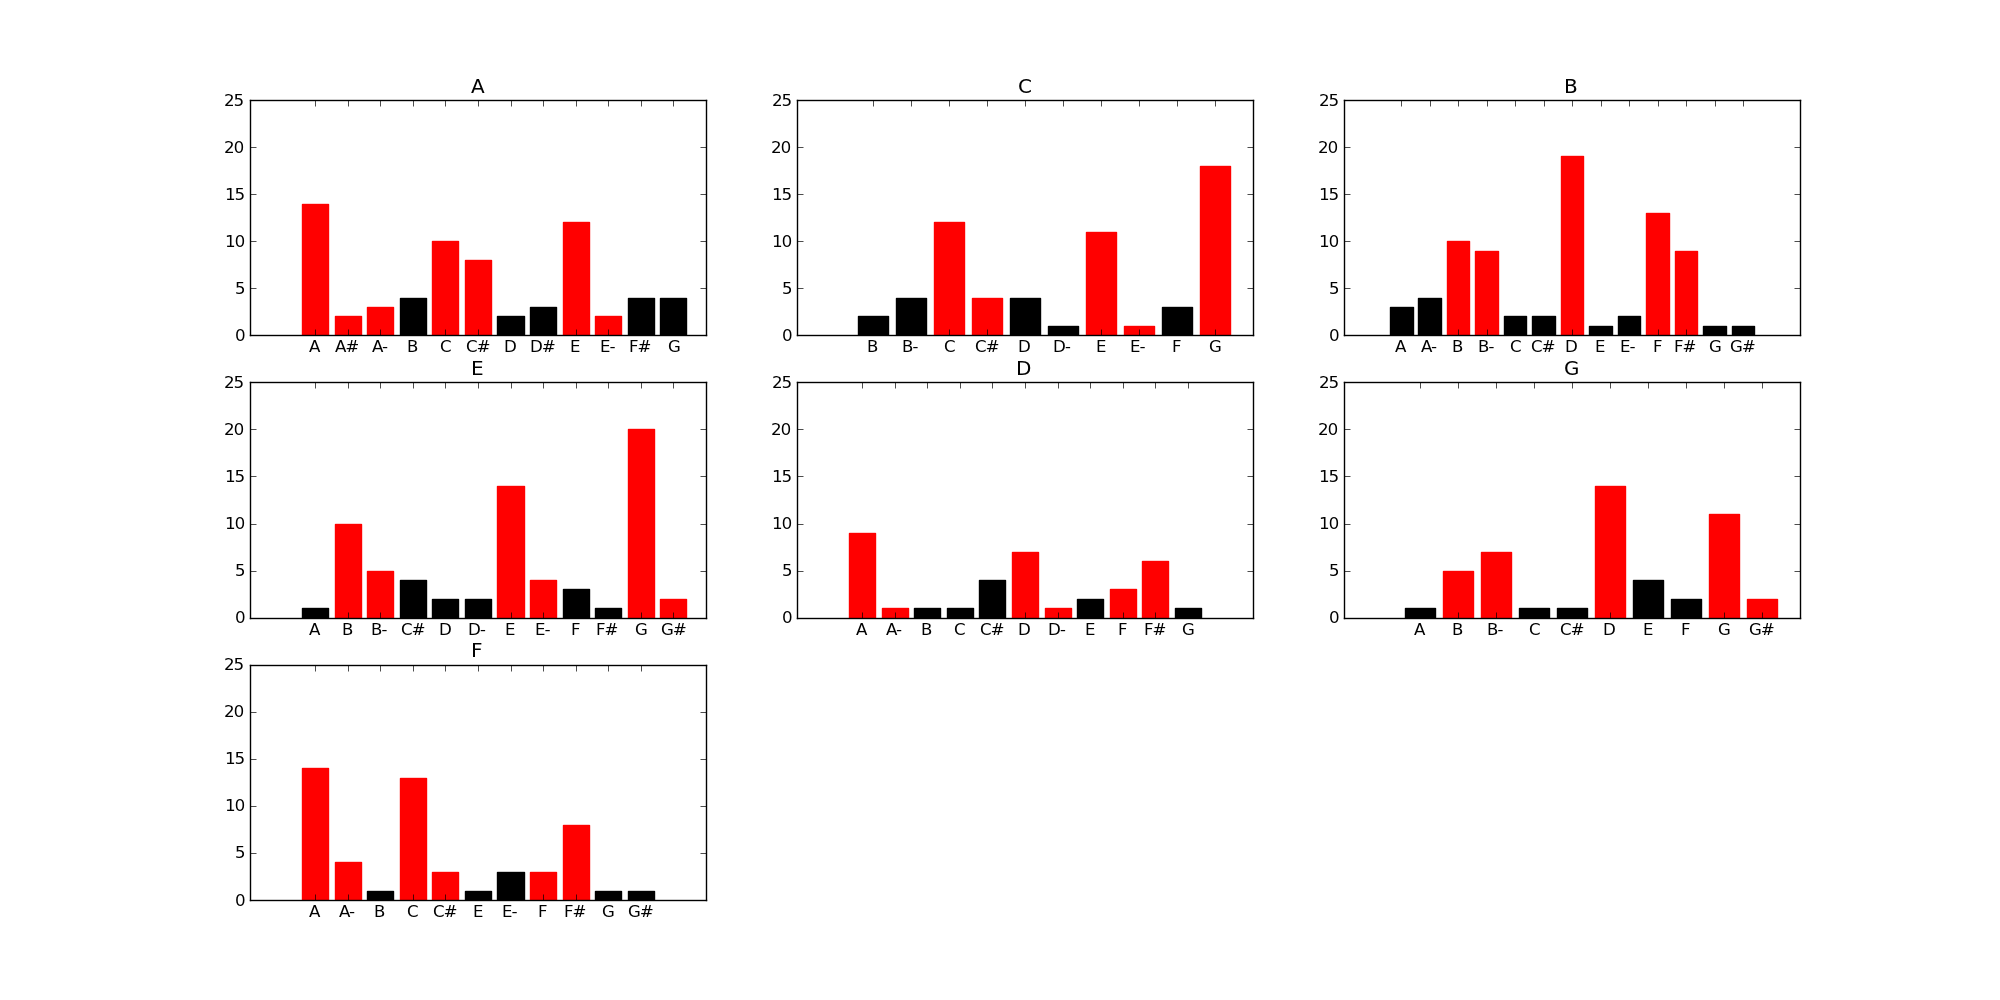
\includegraphics[trim = 220 50 0 0, scale=.45]{pred.png}
\begin{center}\emph{Figure 5: Pitch class error distributions, actual (green) vs prediction (red)}\\ \end{center}

\newpage

Figure 5 shows the number of pitches recognized in each wrongly classified time slice. The green graphs show the distributions under what should have been the classificaiton, and the red graphs show the distributions under what was predicted using an SVM classifier. It can be seen that the triads of each chord (C,E,G for C, for example) tend to have higher counts for both graphs. The counts seem to be comparatively high in the red graphs, however, for triads of distances one and two (E,G for C). This indicates that the majority of misclassifications are due to trouble in disambiguating between chords which are triads apart.  The following graphs demonstrate this as well:

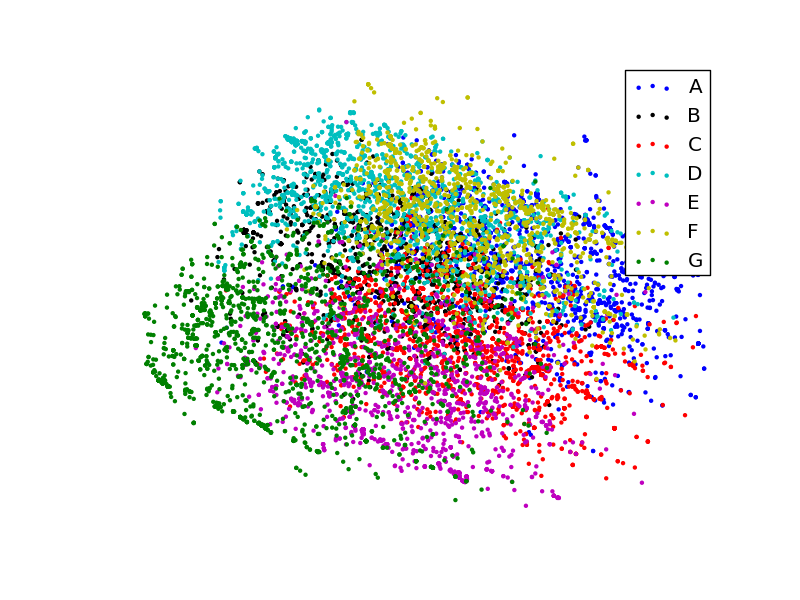
\includegraphics[trim = 70 40 0 00, scale=.85]{pcaFinal.png}\\
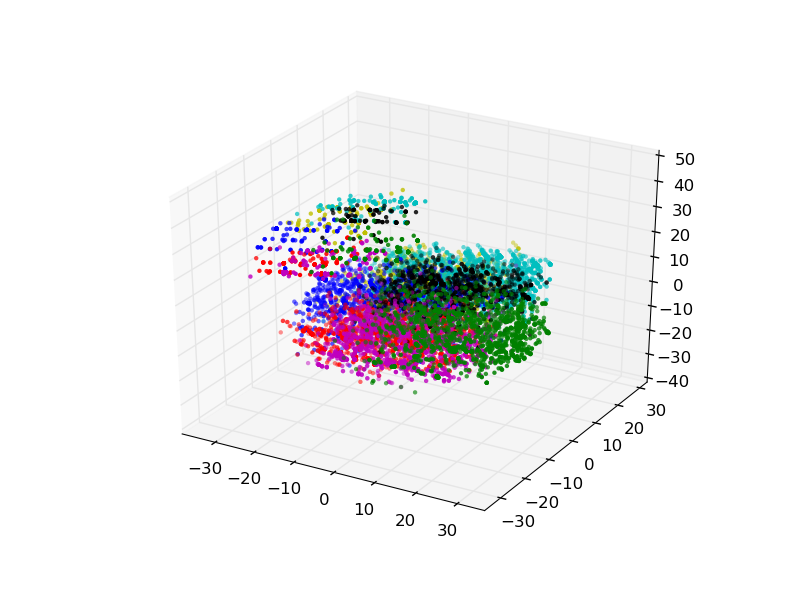
\includegraphics[trim = 70 40 0 35, scale=.85]{markov3d.png}
\begin{center}\emph{Figure 6: Pitch class resultant clustering, 2d/3d dimensionality reduction using PCA}\\ \end{center}

Under both clustering visualizations, we can see that the chords connect with each other in distances of triads. The three-dimensional projection shows this in particular; the chord-root classifications form a ring, of sorts, where each chord connects to those which are triads apart. The ambiguity, then, lies in these interconnections.\\

\begin{center}
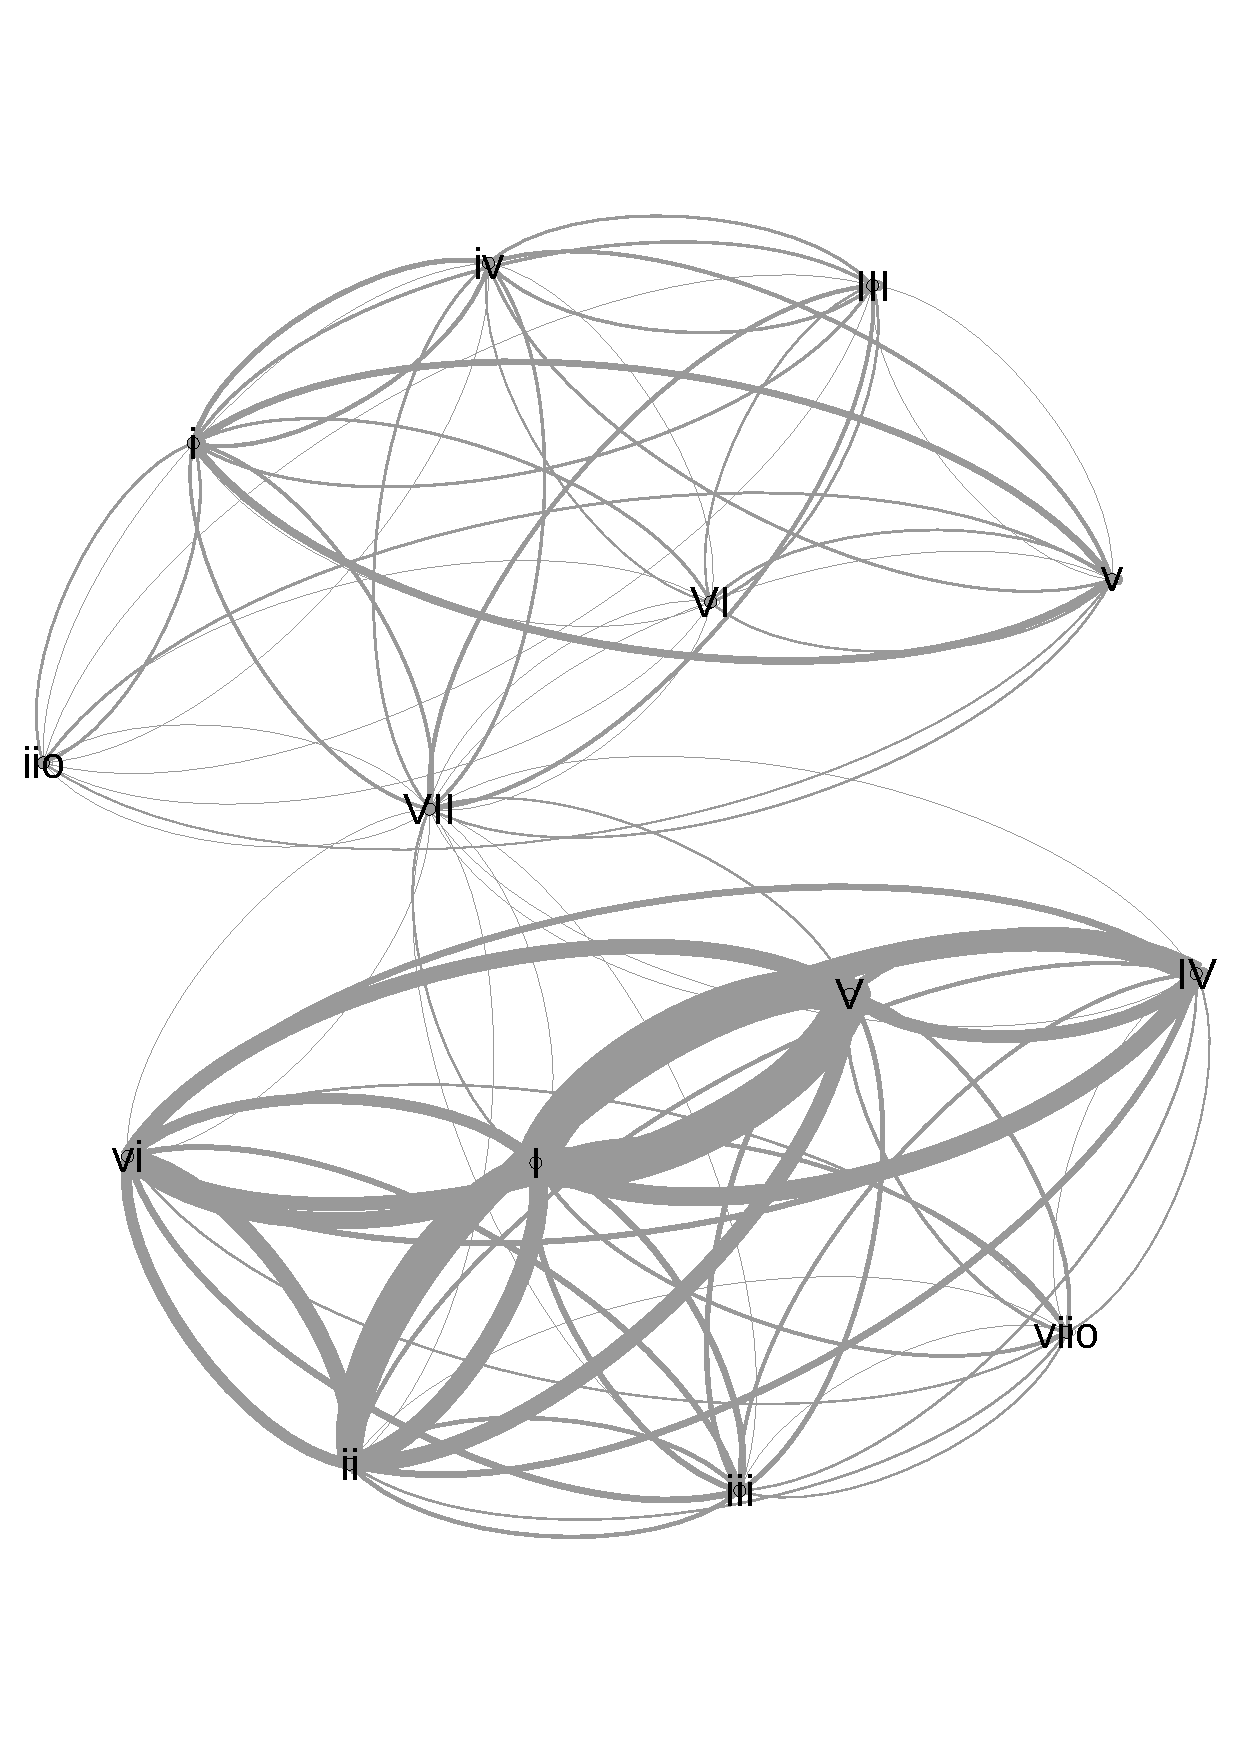
\includegraphics[trim = 0 50 0 40, scale=.25]{markov2.pdf}
\end{center}
\begin{center}\emph{Markov 1st Order Progression Distribution}\\ \end{center}

\begin{center}
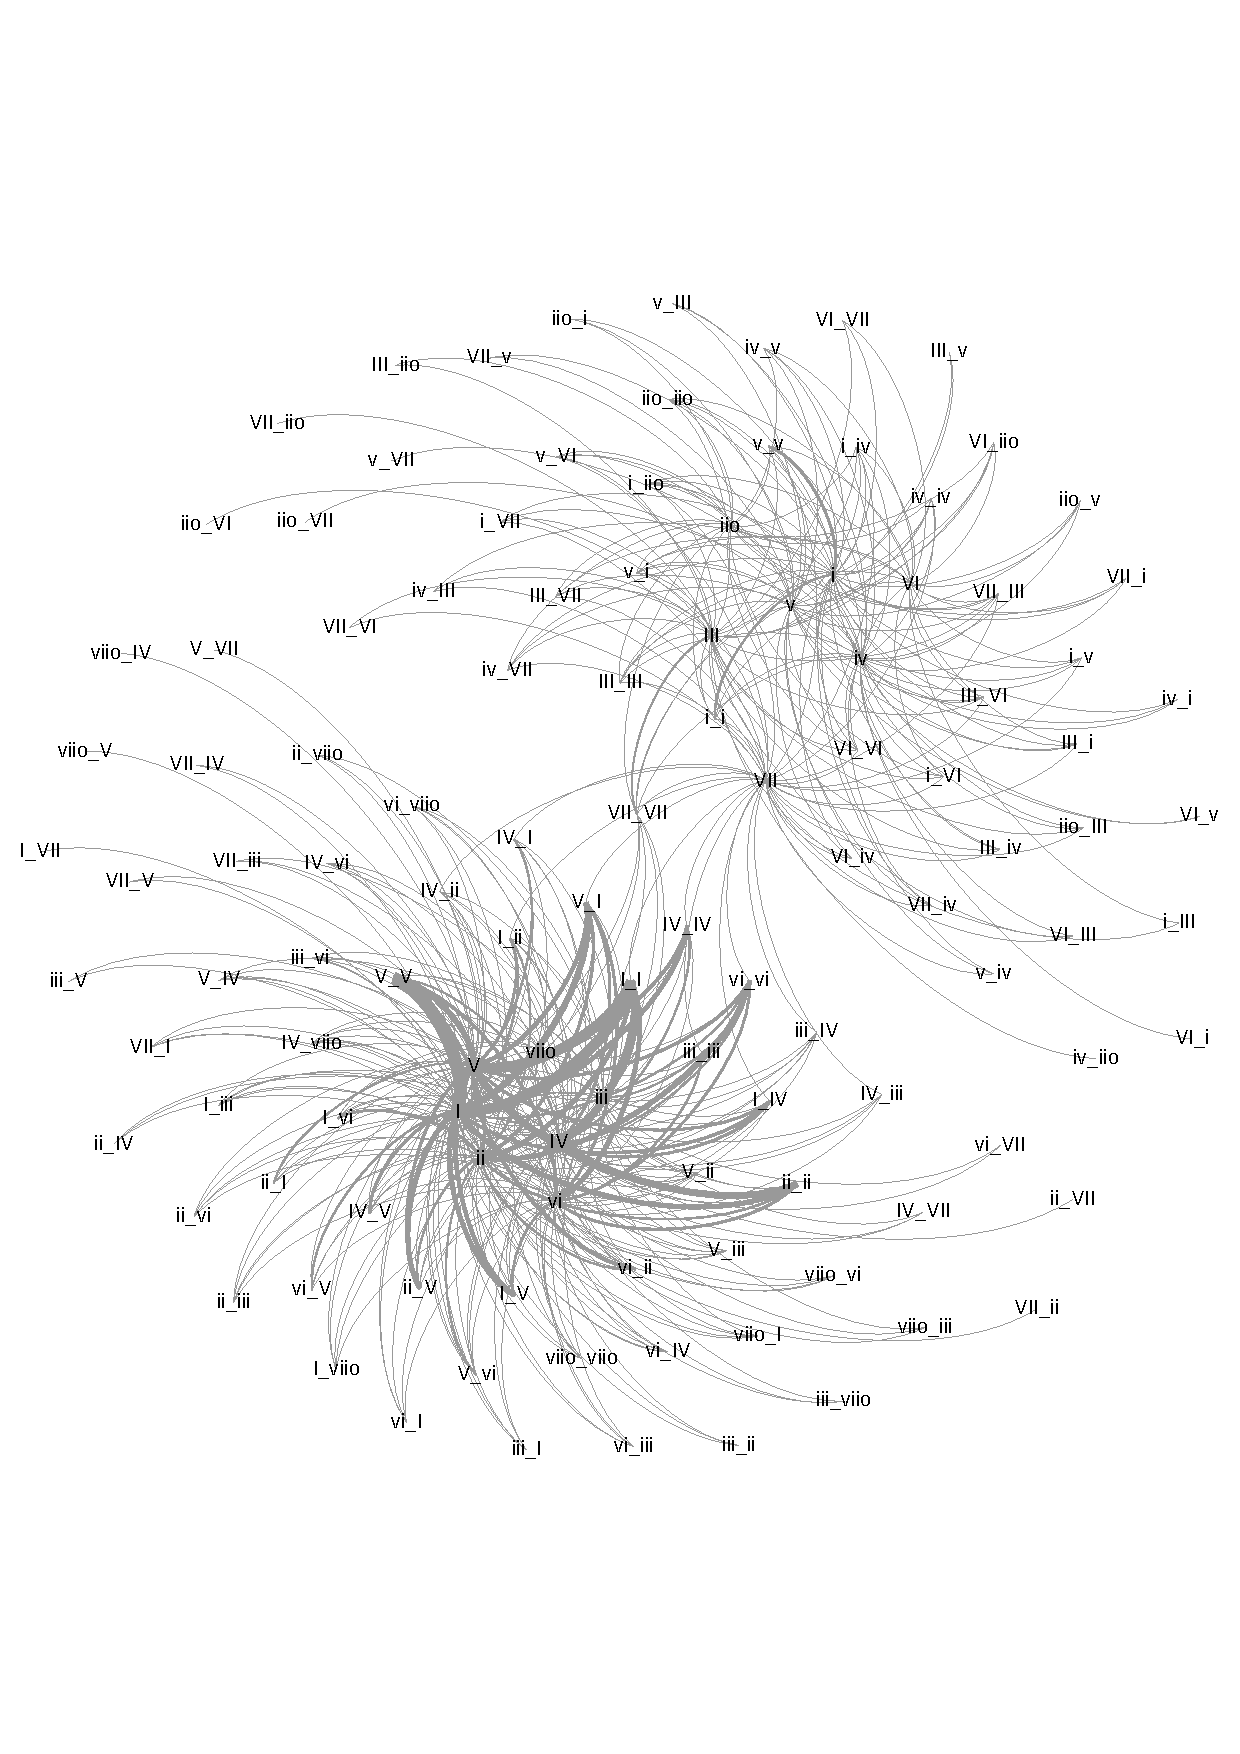
\includegraphics[trim = 0 100 0 100, scale=.75]{markov3.pdf}
\end{center}
\begin{center}\emph{Markov 2nd Order Progression Distribution}\\ \end{center}

\newpage
\begin{center}
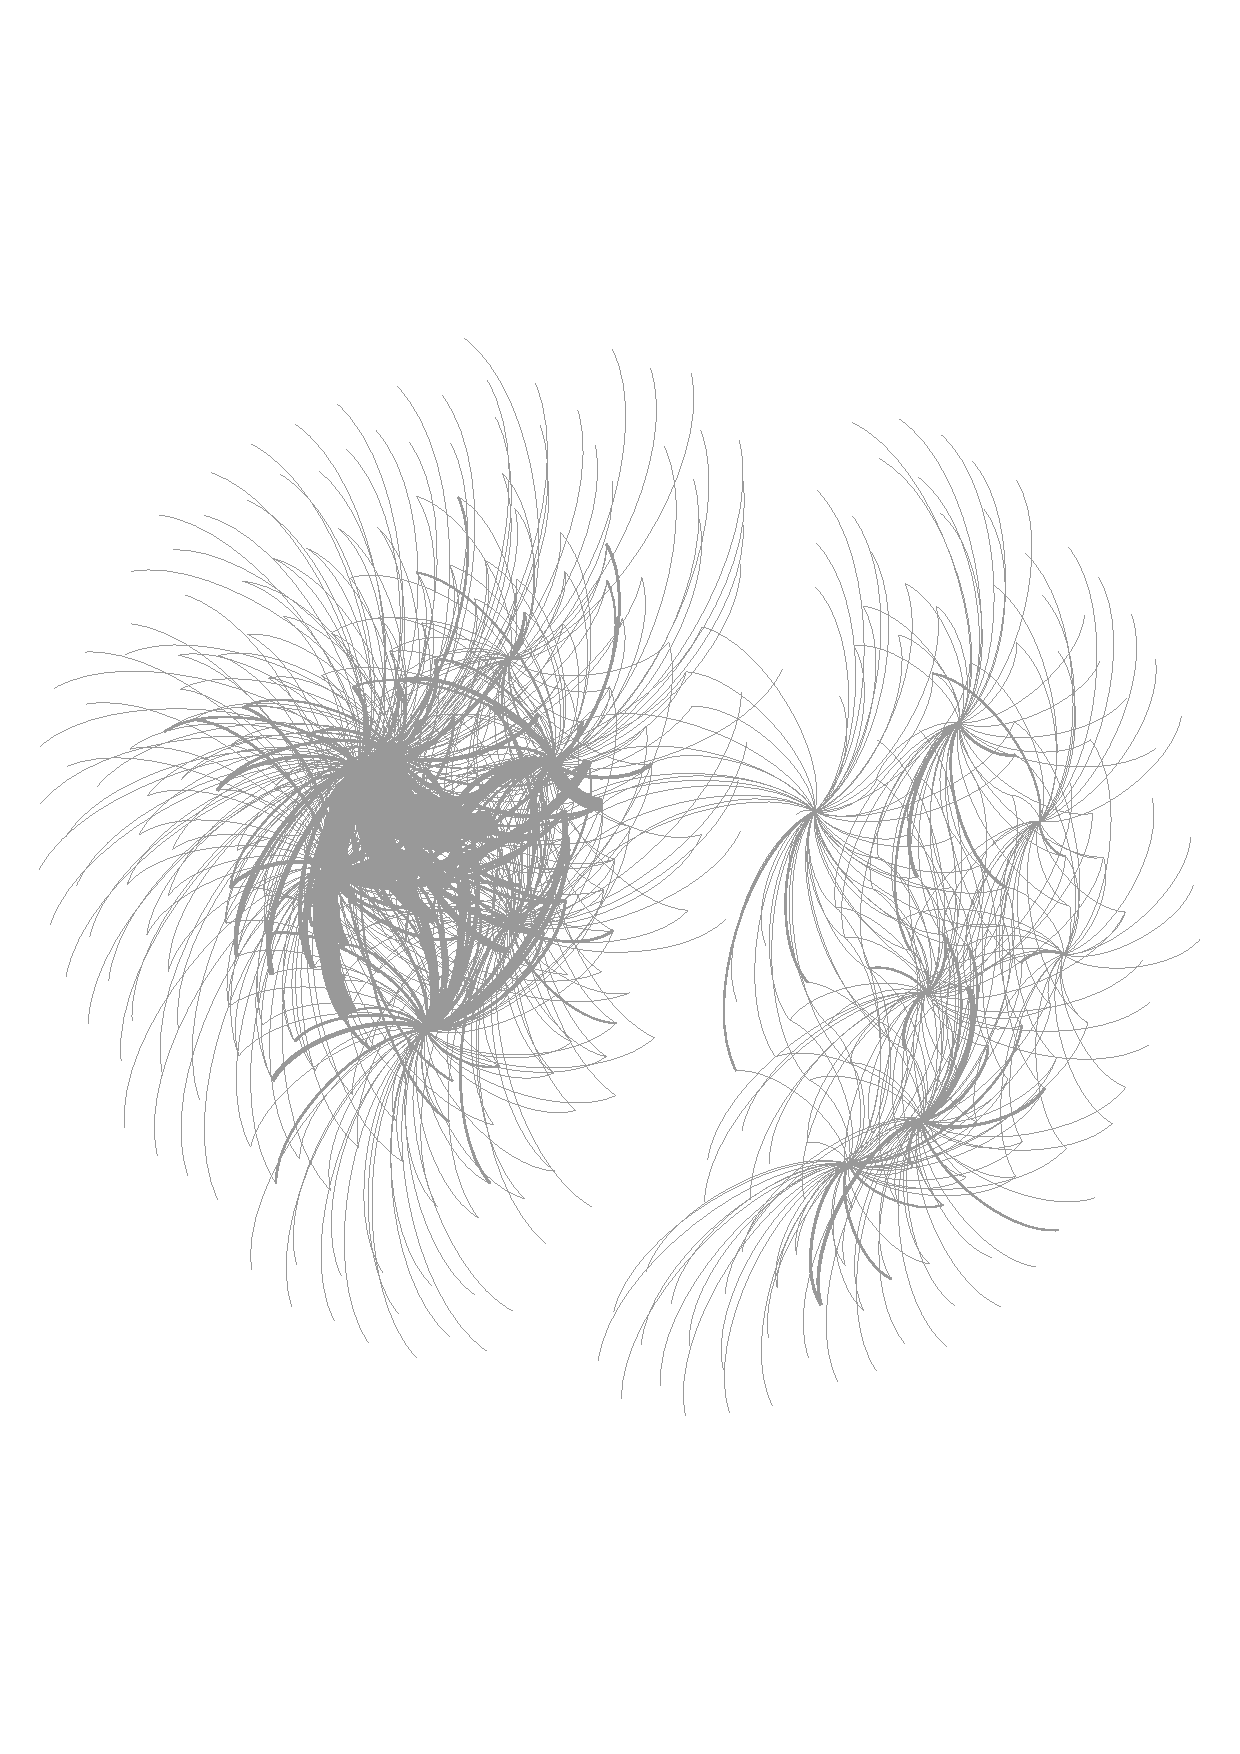
\includegraphics[trim = 0 100 0 100, scale=.5]{markov4.pdf}
\end{center}
\begin{center}\emph{Markov 3rd Order Progression Distribution}\\ \end{center}

The various Markov progressions demonstrate the lopsided progression counts for each chain ordering. The features tended to predict the same base root (adjusted for key) for each incoming progression, which may have been responsible for the poor performance. 

\section{Conclusion}
The different classifiers did not have a significant difference in performance, implying that the problem is not necessarily linear. Other classification methods may be attempted as well, such as $k$-means clustering, and analysis on dimensionality-reduced data, as seen in figure 6; this may help when thinking about the problem intuitively. The accuracy could be improved further by building features which helped resolve the ambiguity of choosing between triads of chords. One such method may be to create a modified Stack of Thirds feature which recognizes passing tones, and removes them from the score.  

\end{document}